\documentclass[12pt, draft, isbabel]{rureport}


\begin{document}

\maketitle

\tableofcontents

\listoffixmes

\clearpage

\section{Inngangur}\label{ch::inngangur}

Markmið verkefnisins er að hanna boltasamsetningu sem halda skal þremur stál stöngum saman. 
Við hönnun skal stærð, fjöldi og staðsetning bolta útfærð svo að samsetningin beri sem mest álag F, álagstilvik er sýnt á mynd \ref{fig::forsendur}. 
Athuga skal að myndin sýnir ekki heppilegt tilvik samsetningar. 

Nota skal 8.8 bolta ($S_y$ = 660 MPa og $S_{ut}$ = 830 MPa) og reikna með að efni í stöngum sé stál AISI 1020 HR ($S_y$ = 210 MPa og $S_{ut}$ = 380 MPa) eða sambærilegt. 
Reikna skal öll möguleg tilvik á að samsetningin eða stangirnar gefi sig. Samsetningin verður síðar prófuð og bera skal útkomu prófunarinnar saman við reiknuð gildi á mestu spennu. 
Ef útkoma prófana stangast á við reiknuð gildi skal gera grein fyrir ástæðum þess. 
Reikna má með því að undirstöðurnar eru staddar 1 cm frá enda stanga.

\begin{figure}[b]
	\centering
	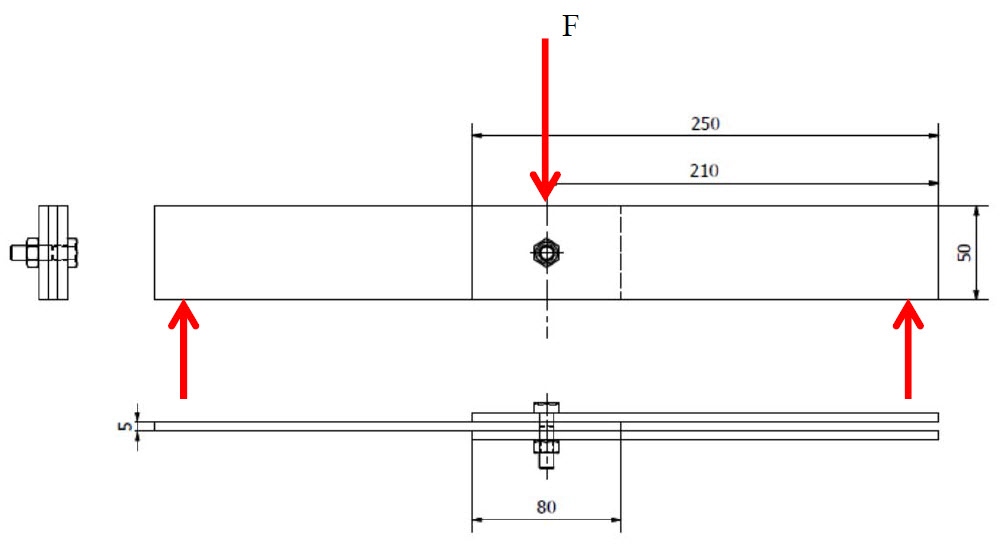
\includegraphics[width=1\textwidth]{forsendur}
	\caption{\fxnote{Veit ekki alveg hvað á að standa hér}}
	\label{fig::forsendur}
\end{figure}

\include{reikningar}


\section{Niðurstöður}
\label{sec:nidurstodur}

Samkvæmt útreikningum okkar hefðu plöturnar gefið sig á undan boltunum eða við $4375 N$, \sbr kafla \ref{ch::reikningar}.
Boltarnir hefðu átt að þola allt að \fxnote{álag sem boltar þola} álag.

\begin{figure}[h]
  \centering
  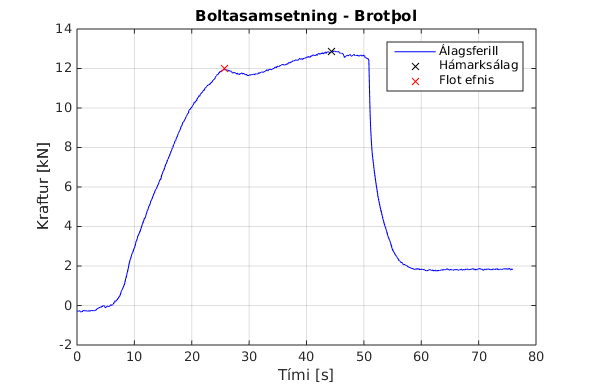
\includegraphics[width=\linewidth]{alag}
  \caption{Álagsferill í þolprófun}
  \label{fig:alag}
\end{figure}

Þar sem útreikningar okkar miðast við eina plötu, \te eftir að aðskilnaður hefur átt sér stað, er þetta ekki alveg rétt.
Ef reiknað væri með öllum plötunum, þ.e.~áður en aðskilnaður hefur átt sér stað, myndi flatartregðuvægið þrefaldast, sem passar nokkuð vel við þau gildi sem komu fram í prófunum.
Eins og sjá má á mynd \ref{fig:alag} kemst efnið í flot við \(12 kN \approx 4375 N \cdot 3 = 13.13 kN\) sem stenst nokkuð vel.
Skekkjan á því er þá \(100\% - {12 \over 13.13} = 8.61\% \)

\clearpage

\begin{figure}
  \centering
  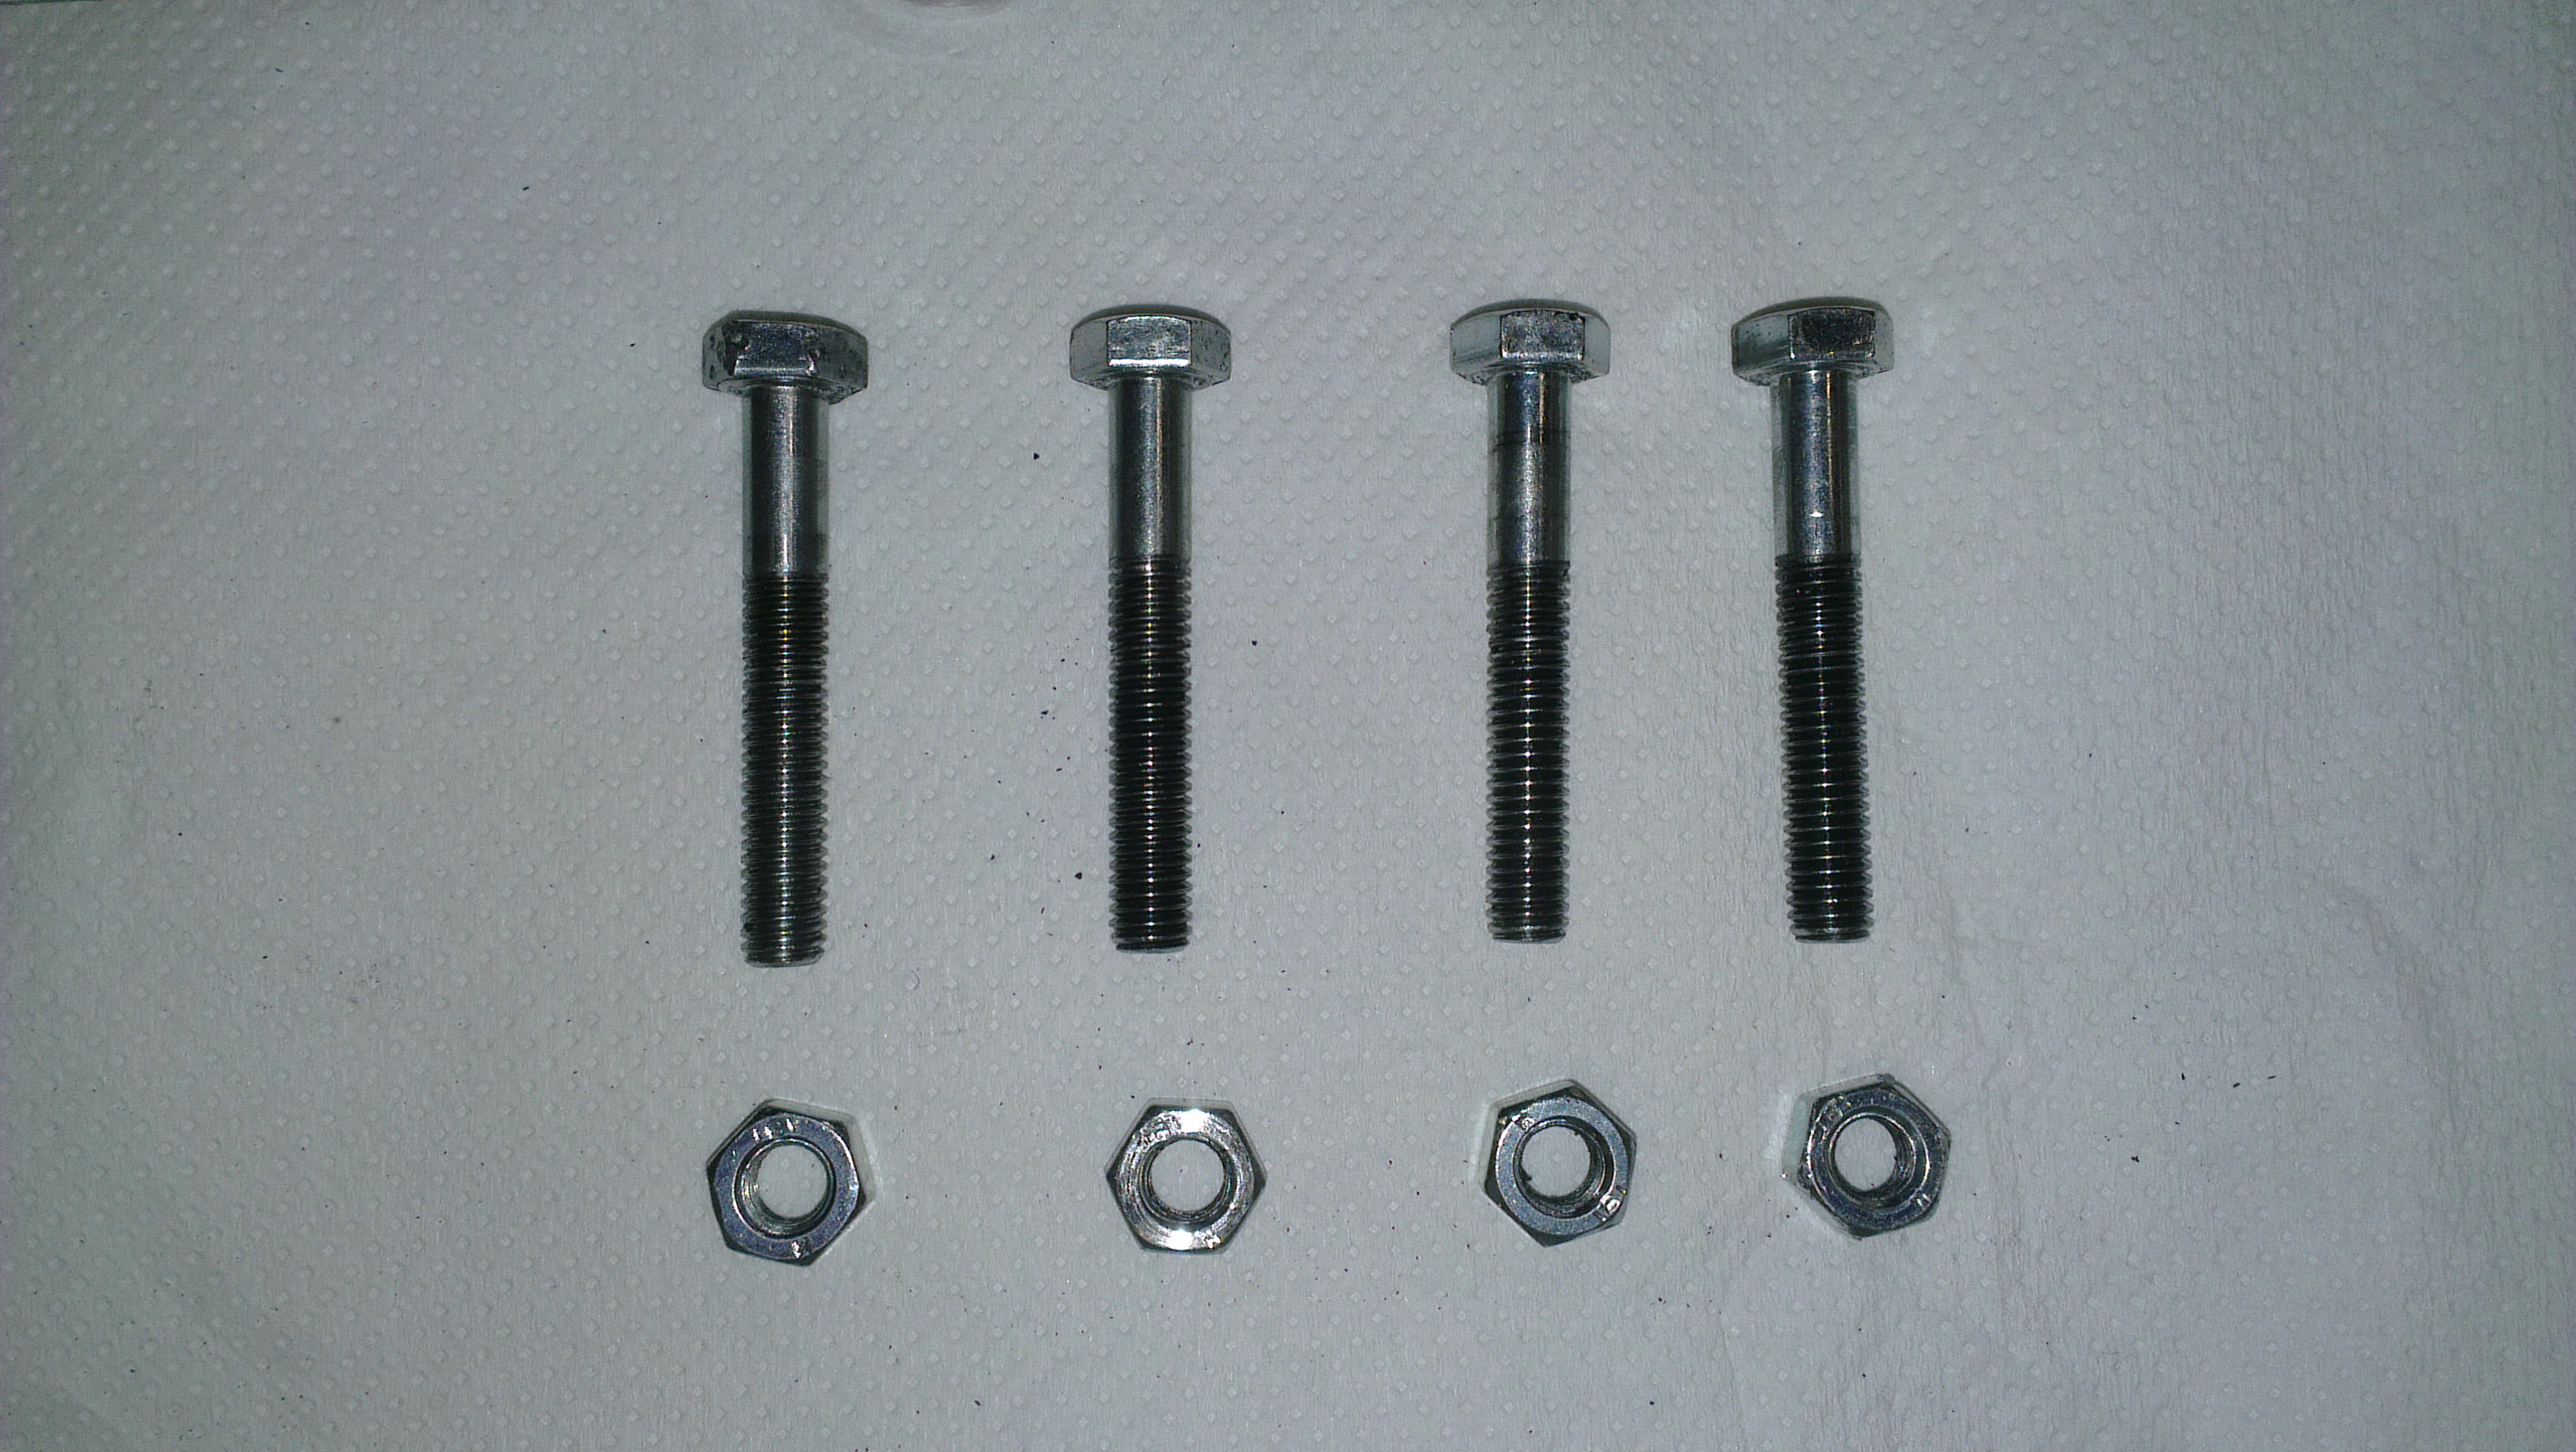
\includegraphics[width=\linewidth]{boltar}
  \caption{Boltar eftir prófun}
  \label{fig:boltar}
\end{figure}

\begin{figure}
  \centering
  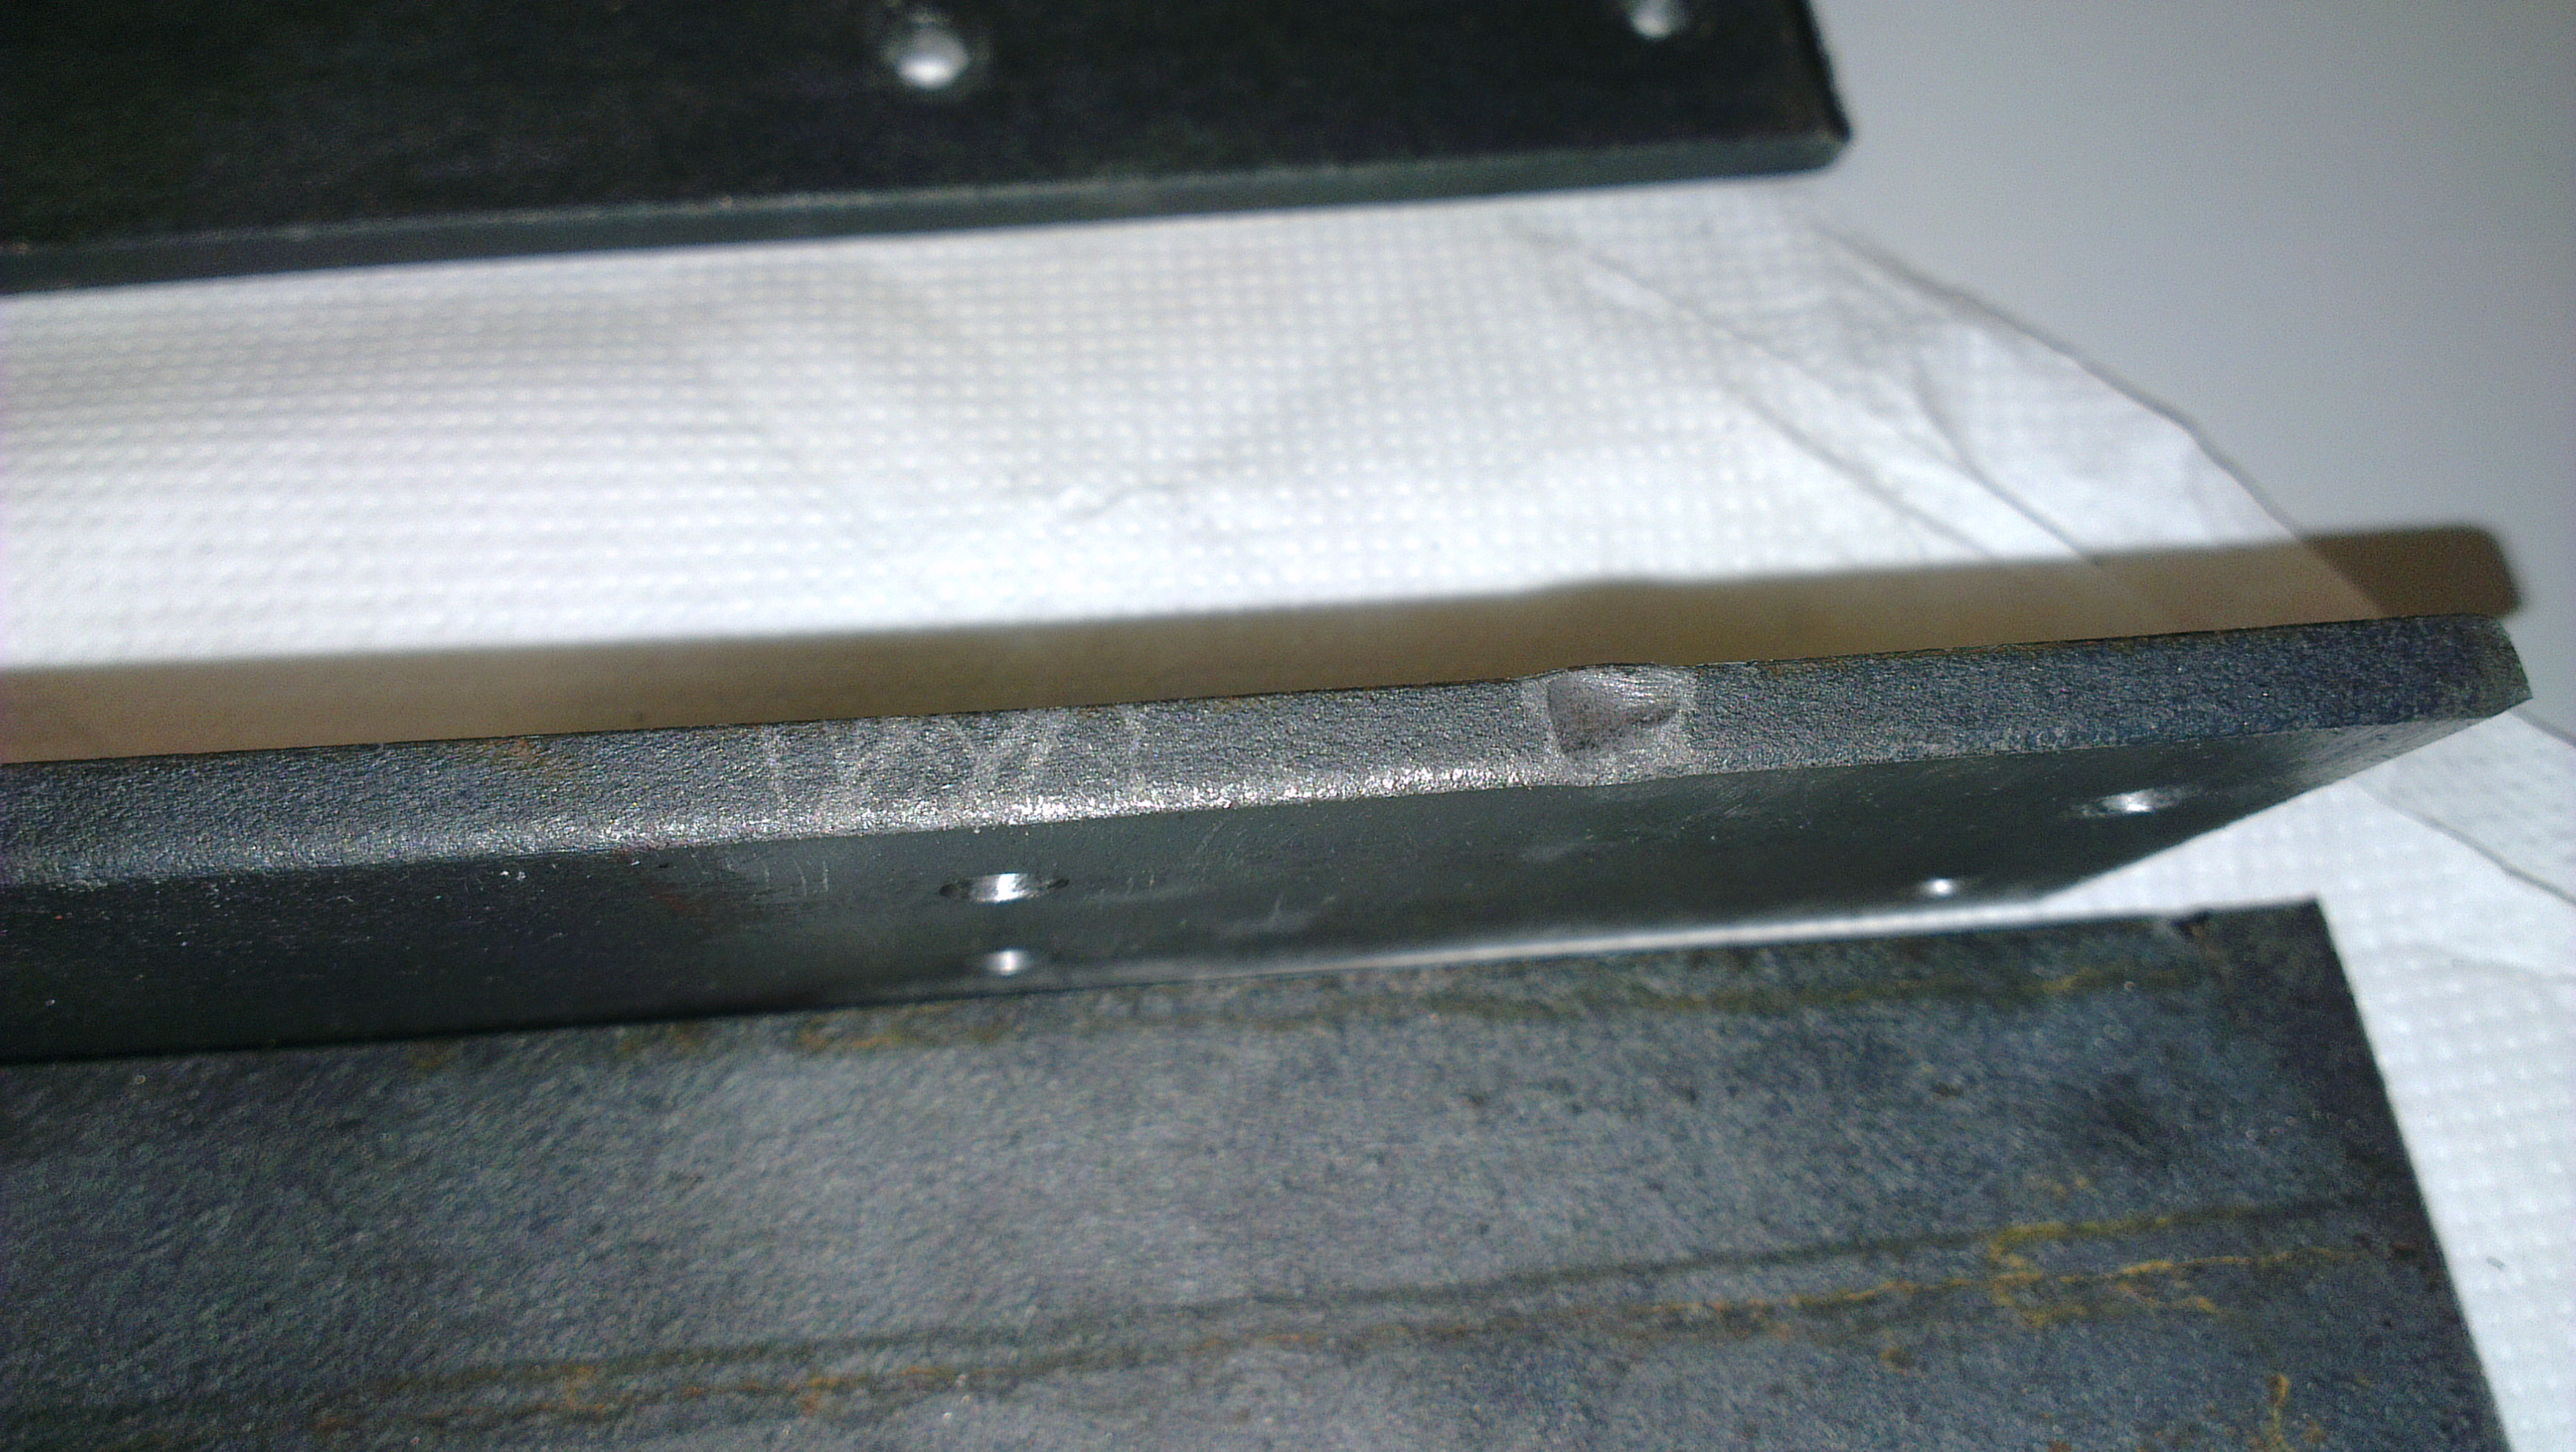
\includegraphics[width=\linewidth]{hak}
  \caption{Hak sem myndaðist í einni stöng við prófun}
  \label{fig:hak}
\end{figure}

\begin{figure}
  \centering
  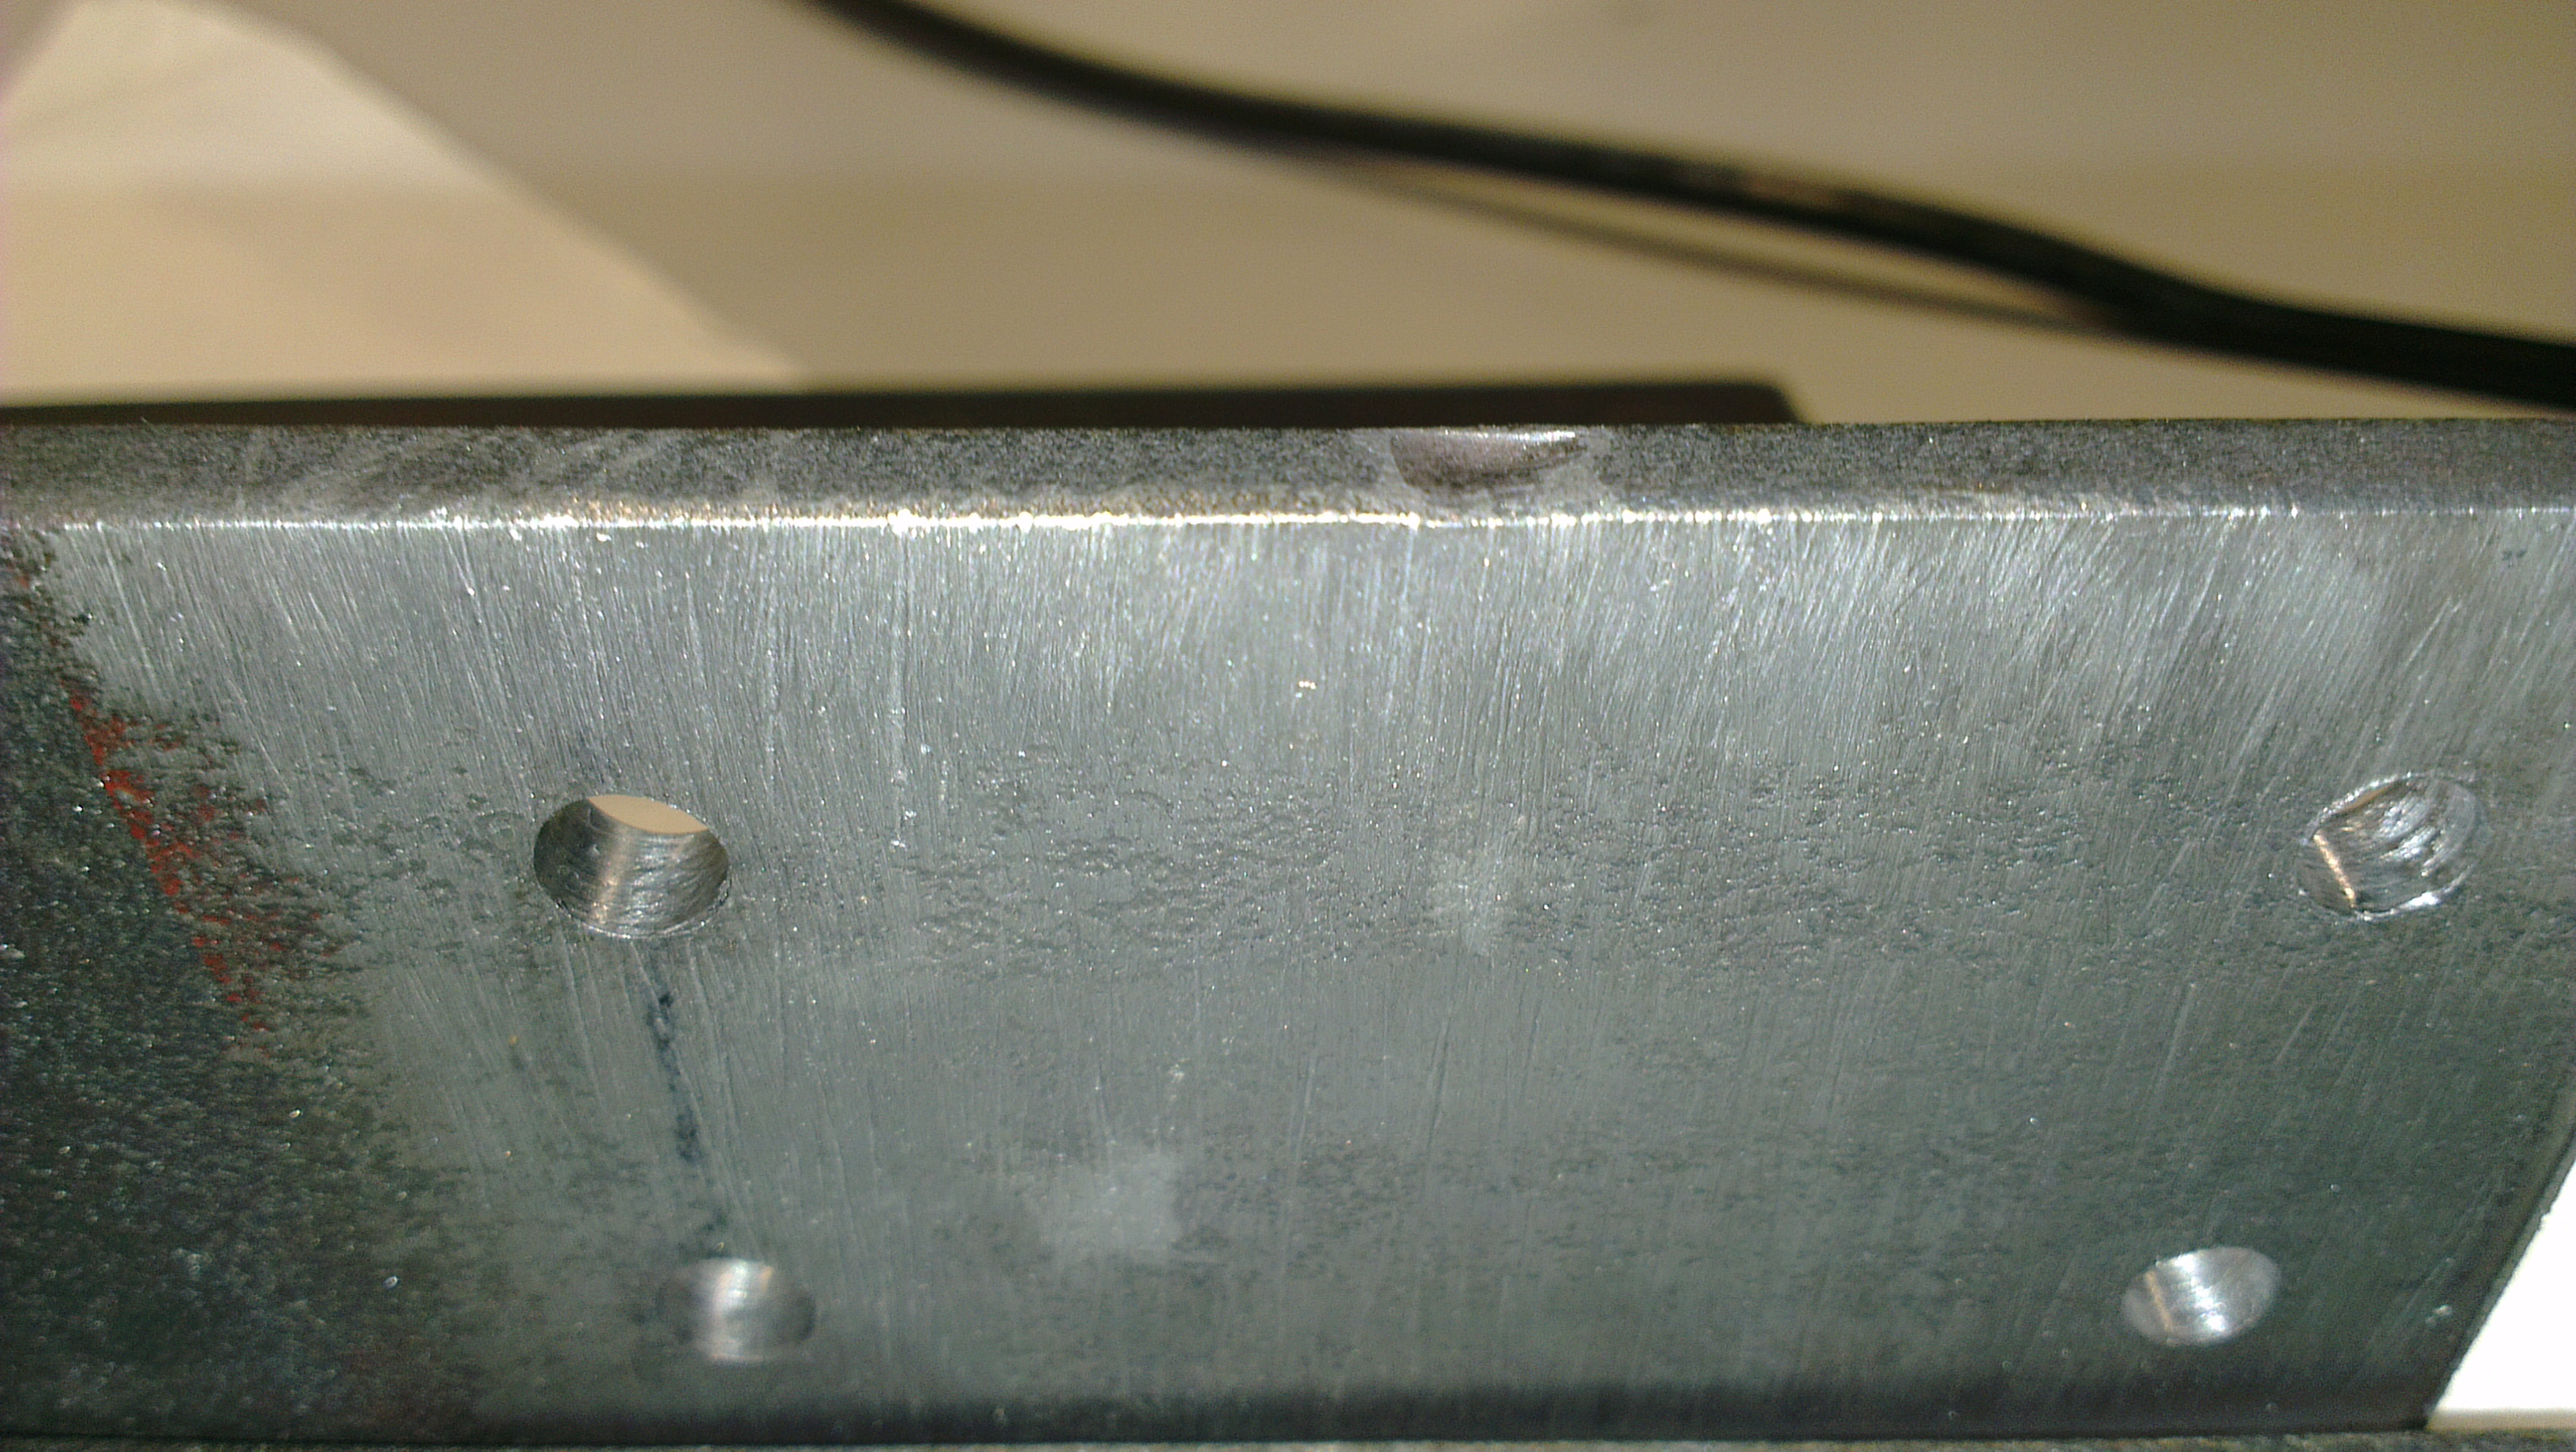
\includegraphics[width=\linewidth]{hak2}
  \caption{Hak sem myndaðist í einni stöng við prófun}
  \label{fig:hak2}
\end{figure}


\begin{figure}
  \centering
  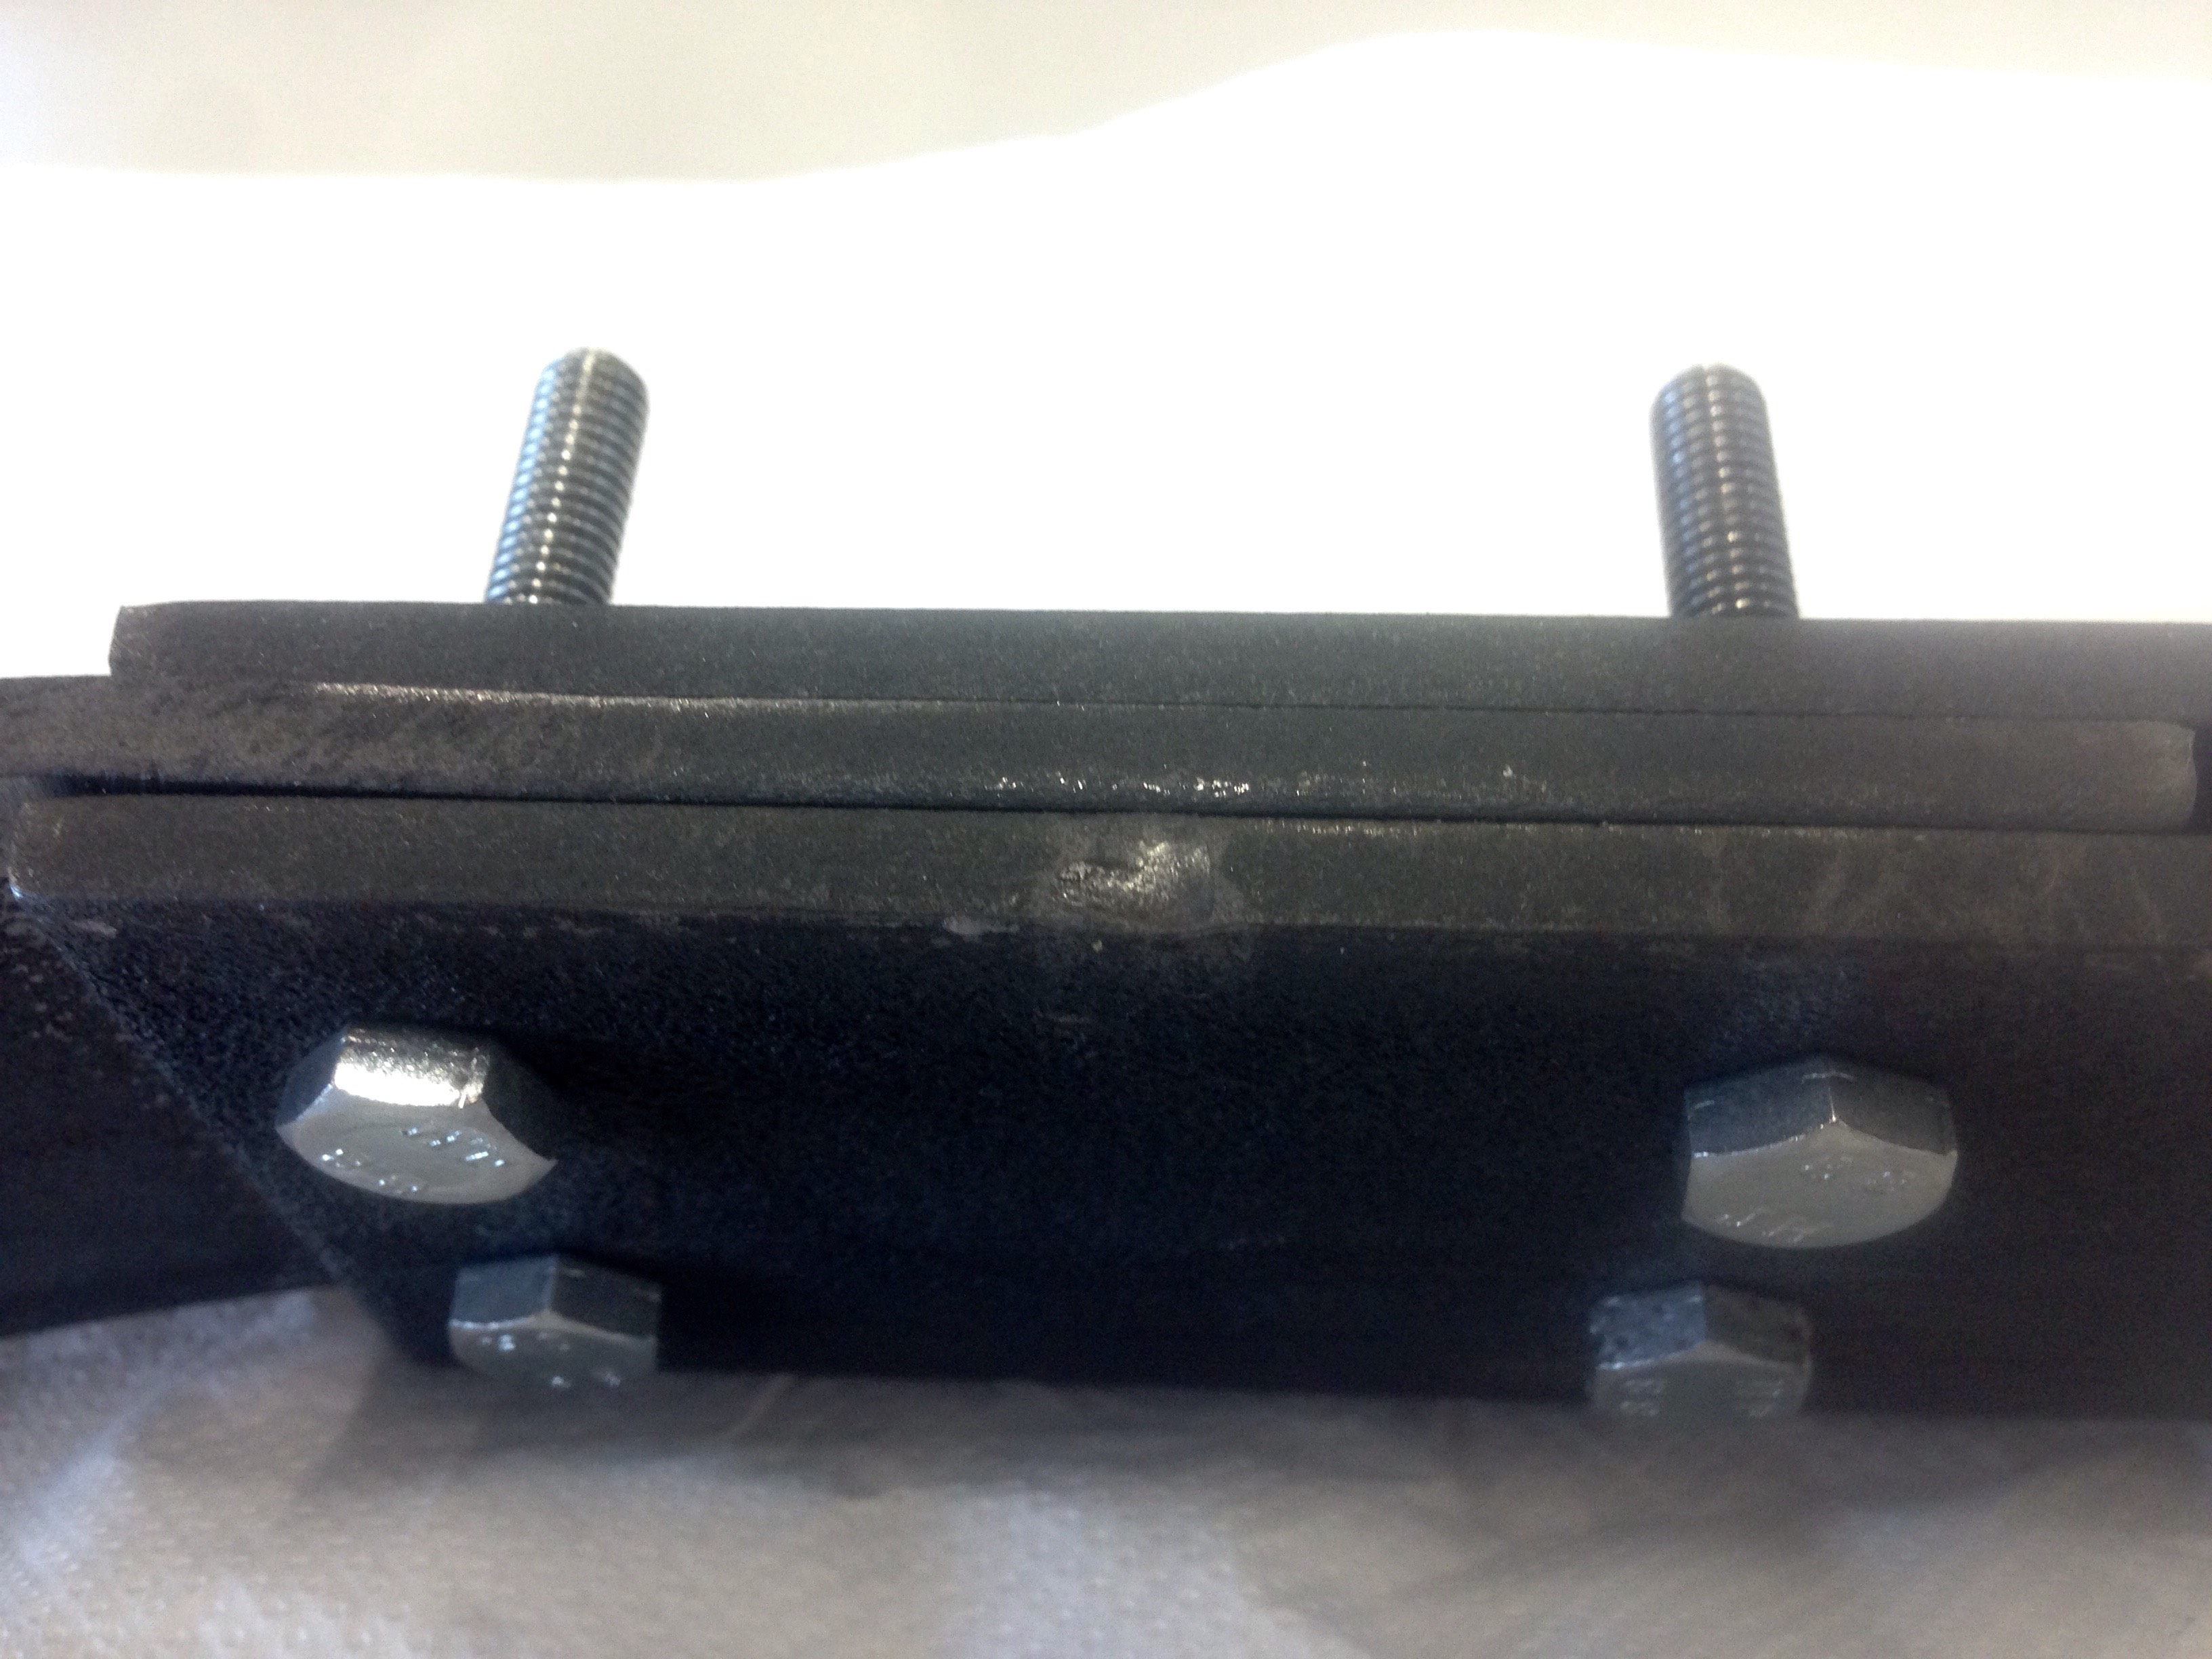
\includegraphics[width=\linewidth]{hak4}
  \caption{Hak sem myndaðist í einni stöng við prófun}
  \label{fig:hak4}
\end{figure}



Við álagsprófið beygluðust stálplöturnar en ekkert sá á boltunum, sbr. myndir \ref{fig:boltar}, \ref{fig:pano} og \ref{fig:exploded}.
Auk þess má sjá á stálplötunum að álagið var að mestu leyti á eina af ytri plötunum, sbr. myndir \ref{fig:hak}, \ref{fig:hak2} og \ref{fig:hak4}, og því var átakið skakkt. Þetta olli því að meira af álaginu fór í stálplöturnar, en minna af álaginu í boltana.
Það olli því að plöturnar beygluðust áður en nægt átak færi í boltana til að valda einhverju teljanlegu átaki á boltana.

\clearpage

\begin{figure}
  \centering
  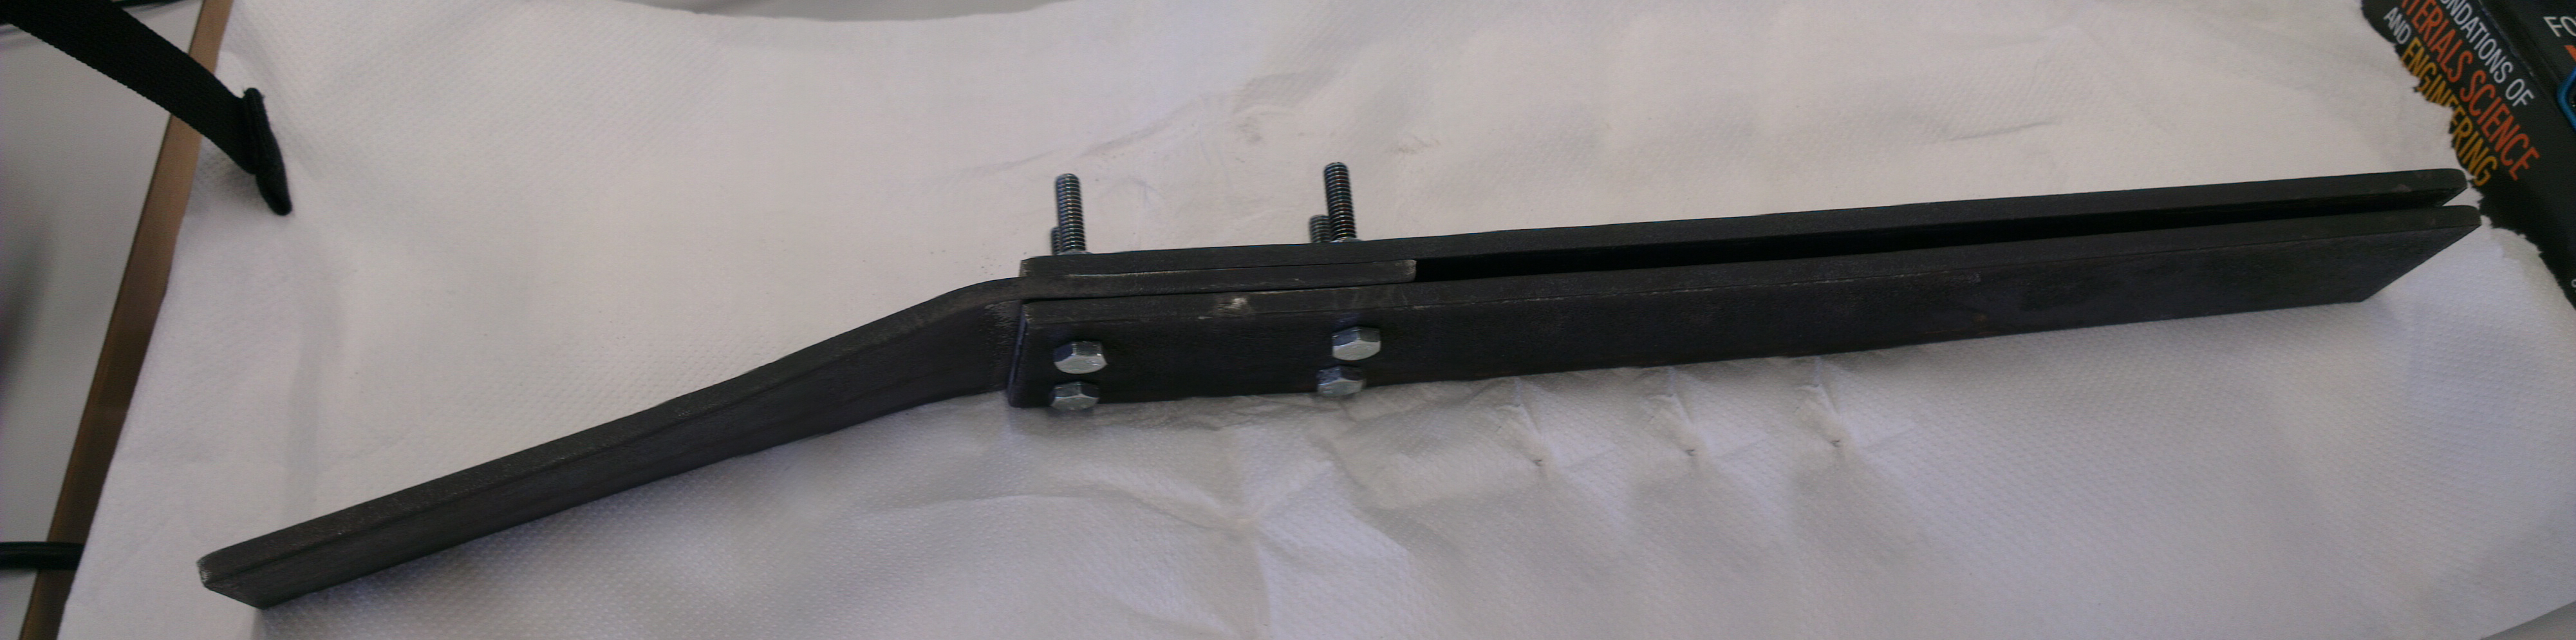
\includegraphics[width=\linewidth]{beygja_pano}
  \caption{Samsetning eftir prófun}
  \label{fig:pano}
\end{figure}


\begin{figure}
  \centering
  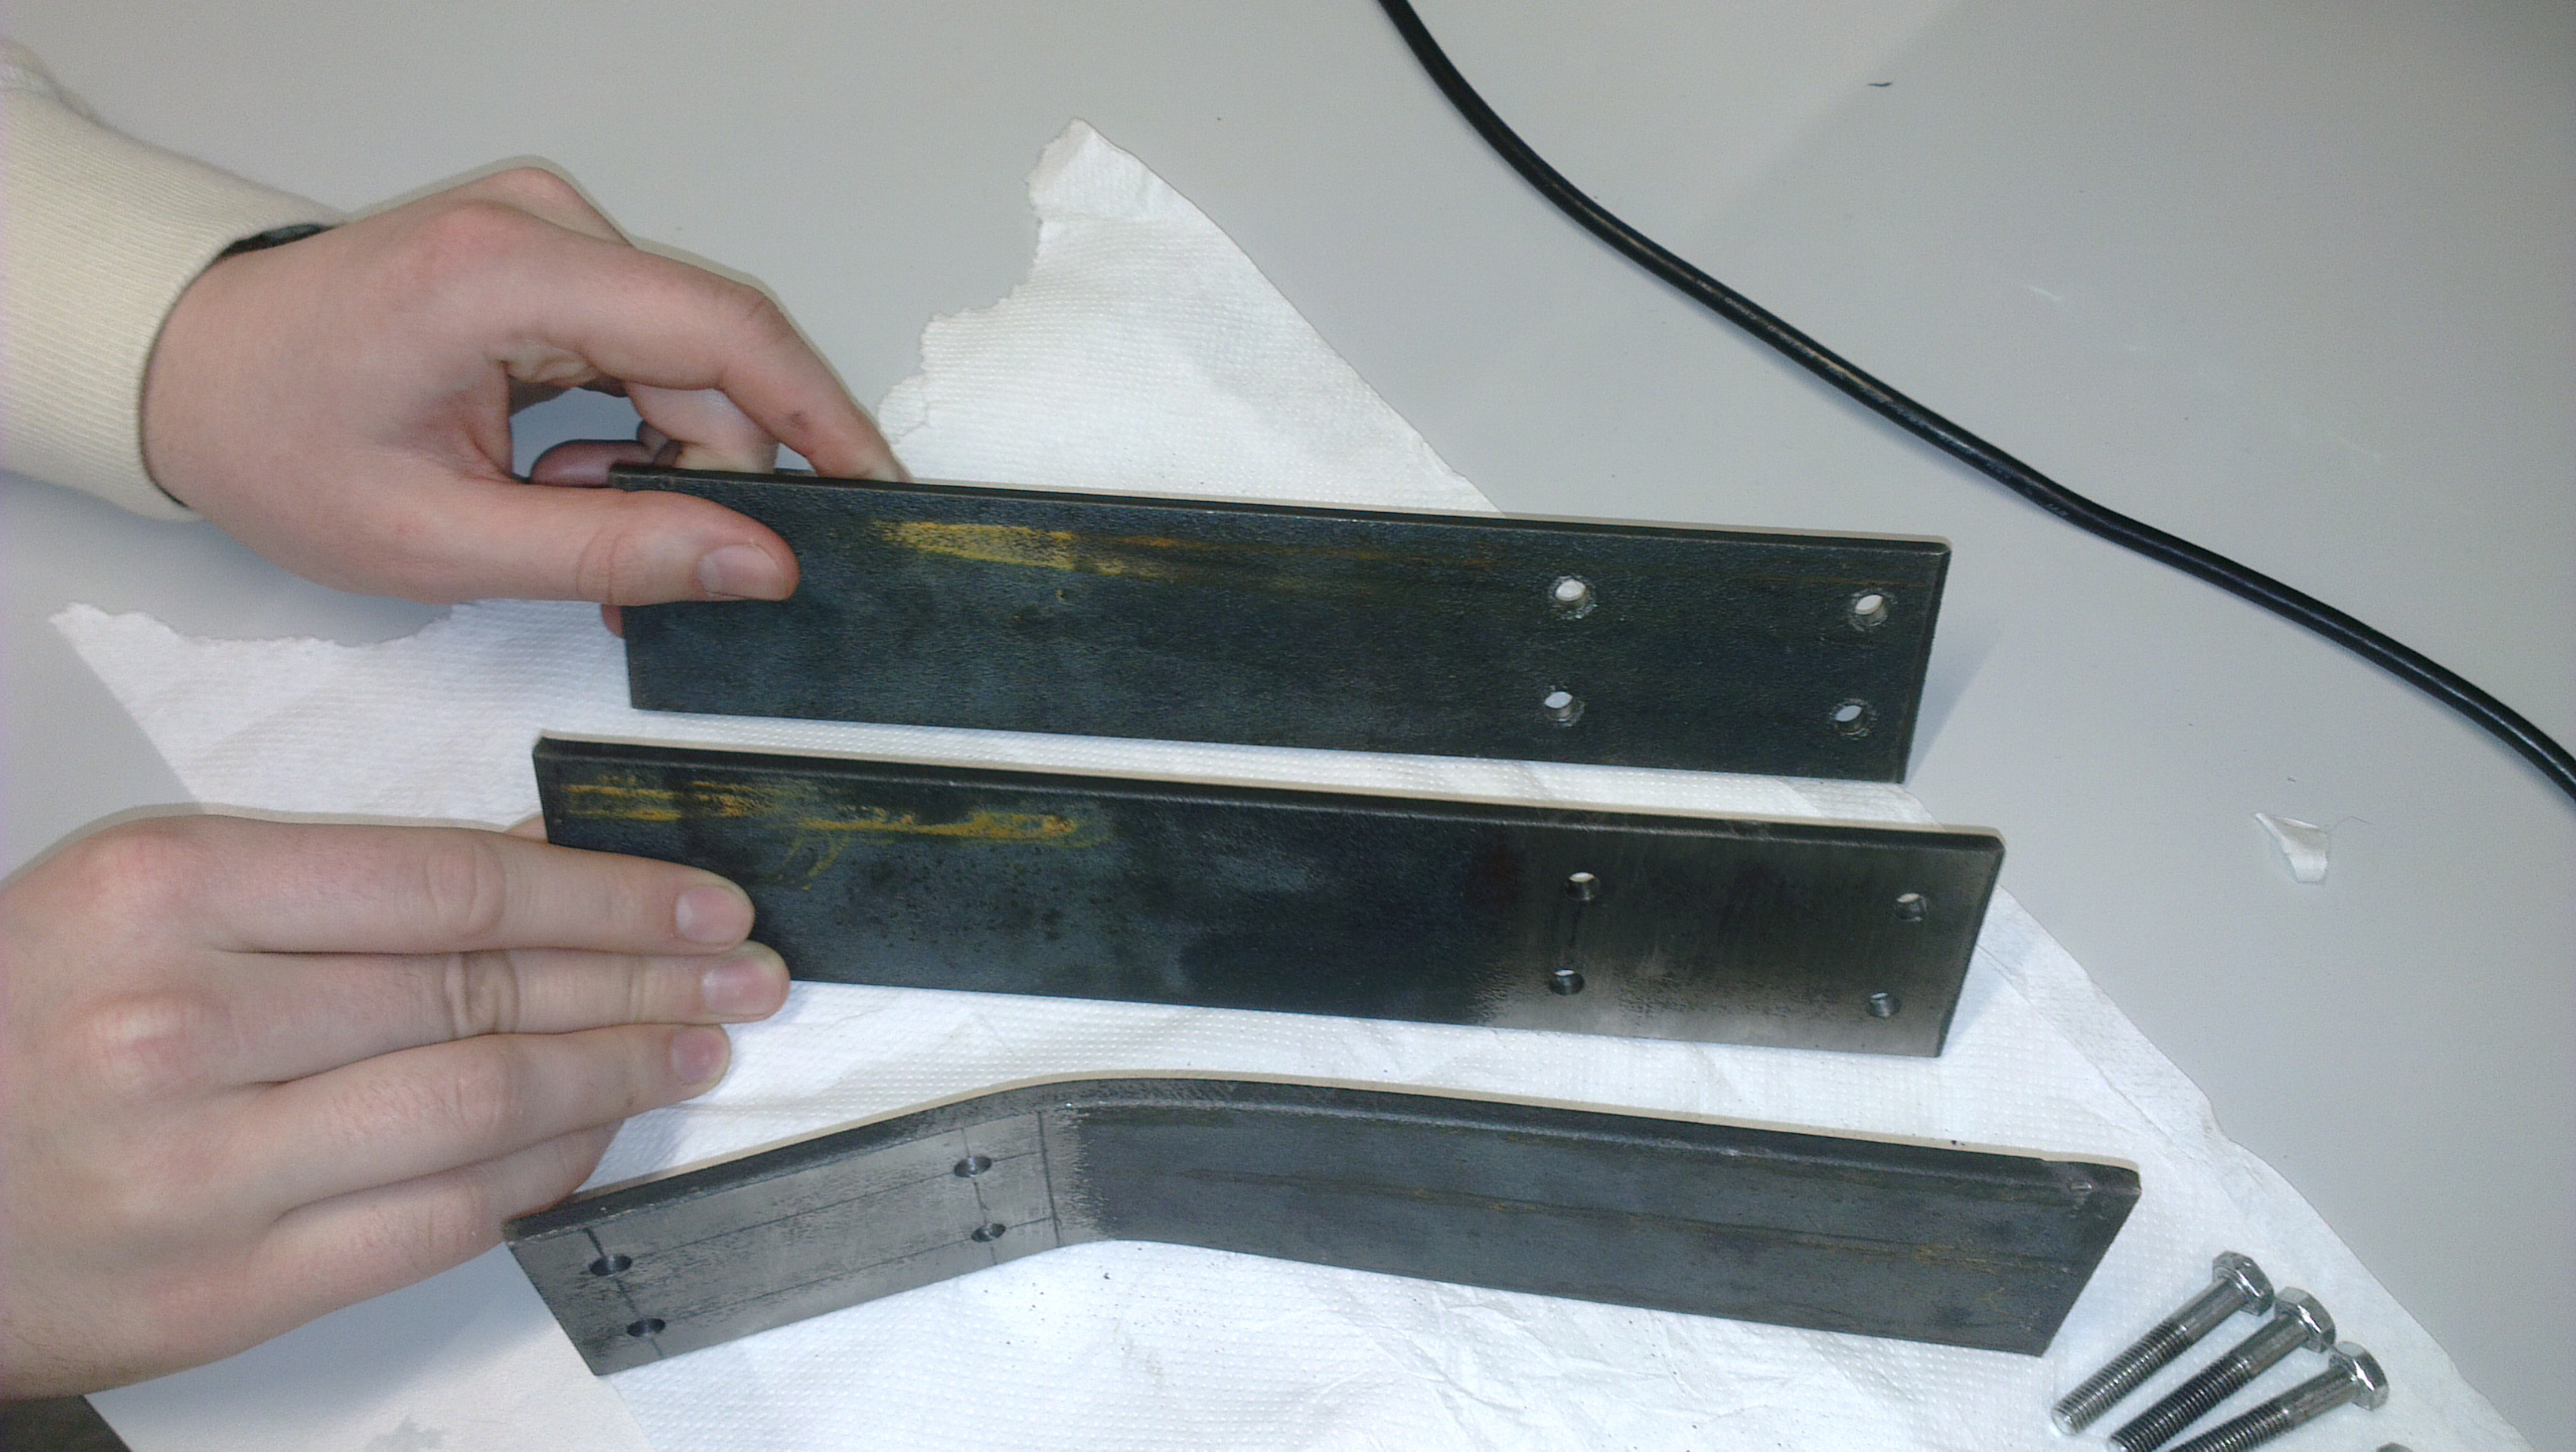
\includegraphics[width=\linewidth]{exploded_view}
  \caption{Tekið sundur eftir prófun}
  \label{fig:exploded}
\end{figure}

Því má í rauninni segja að prófið hafi verið gallað þar sem tækin voru ekki nógu nákvæm til að setja álagið beint í boltana. Það olli því að plöturnar gáfu ekki eftir eins og við gerðum ráð fyrir.

\printbibliography

\end{document}\\
